\subsection{Limits and Continuity}

\subsubsection{Limit Definition}
The limit of a function at a point is the value that function approaches, regardless of whether it actually achieves that value. This makes limits particularly useful for determining what a function does at places it is not defined.\\
For example, the function $\frac{x^2+4x+3}{x+1}$ is undefined at $x=-1$, however, we can take the limit as $x$ approaches $-1$ to see what value the function approaches:
\begin{align*}
    \lim \limits_{x\to -1}\frac{x^2+4x+3}{x+1}\\
    f(-1.1)= 1.9\\
    f(-0.9)= 2.1\\
    f(-1.01)= 1.99\\
    f(-0.99)= 2.01
\end{align*}
As we can see, as we get closer and closer to $x=-1$ the value of $f(x)$ approaches $2$ so we can say that $\lim \limits_{x\to -1}\frac{x^2+4x+3}{x+1}=2$\\
\\
The limit of a function exists such that if $\lim\limits_{x\to a}f(x)=L$ there exists a positive number $\delta$ such that $|f(x)-L|<\varepsilon$ is true for $|x-a|<\delta$\\
Ex: Determine if $\lim\limits_{5x-3}=2$
\begin{align*}
    &f(x)=5x-3,\,a=1,\,L=2\\
    &|x-1|<\delta\\
    &|5x-3-3|<\varepsilon\\
    &|5x-5|<\varepsilon\\
    &5|x-1|<\varepsilon\\
    &|x-1|<\frac{\varepsilon}{5}\\
    &\Ra\delta=\frac{\varepsilon}{5}
\end{align*}
More conceptually, we can say that a limit exists if the right hand and left hand limits approach the same value.\\
i.e. $\lim\limits_{x\to a^+}f(x)=\lim\limits_{x\to a^-}f(x)$\\
Ex: $\lim\limits_{x\to 0^+}\frac{1}{x}=\infty$\\
but $\lim\limits_{x\to 0^-}\frac{1}{x}=-\infty$\\
$\therefore\,\lim\limits_{x\to 0}\frac{1}{x}$ does not exist\\
Ex2: $\lim\limits_{x\to 0^+}\frac{1}{x^2}=\infty$\\
and $\lim\limits_{x\to 0^-}\frac{1}{x^2}=\infty$\\
$\therefore\,\lim\limits_{x\to 0}=\infty$

\subsubsection{Limit Arithmetic}
With limits, we have the following properties:\\
For $\lim\limits_{x\to a}f(x)=l$ and $\lim\limits_{x\to a}g(x)=M$
$$\lim_{x\to a}(f(x)\pm g(x))=\lim_{x\to a}f(x)\pm\lim_{x\to a}g(x)=L\pm M$$
$$\lim_{x\to a}(cf(x))=c\lim_{x\to a}f(x)=cL$$
$$\lim_{x\to a}(f(x)g(x))=\lim_{x\to a}f(x)\lim_{x\to a}g(x)=LM$$
$$\lim_{x\to a}\left(\frac{f(x)}{g(x)}\right)=\frac{\lim\limits_{x\to a}f(x)}{\lim\limits_{x\to a}g(x)}=\frac{L}{M}$$
$$\lim_{x\to a}(f(x))^n=(\lim_{x\to a}f(x))^n=L^n$$
$$\lim_{x\to a}\sqrt[n]{f(x)}=\sqrt[n]{\lim_{x\to a}f(x)}=\sqrt[n]{L}$$
$$\lim_{x\to a}e^{f(x)}=e^{\lim\limits_{x\to a}f(x)}=e^L$$
\\
Limits at Infinity:\\
Ex: $\lim\limits_{x\to\infty}\frac{1}{x}=0$\\
Ex2: $\lim\limits_{x\to\infty}\frac{2x^2}{5x^2-3}$
\begin{align*}
    &=\lim\limits_{x\to\infty}\frac{2x^2}{5x^2-3}\left(\frac{1/x^2}{1/x^2}\right)\\
    &=\lim\limits_{x\to\infty}\frac{2}{5-\frac{3}{x^2}}\\
    &=\frac{2}{5}
\end{align*}
Ex3: $\lim\limits_{x\to-\infty}\frac{x+6}{\sqrt{16x^2-7}}$
\begin{align*}
    &=\lim\limits_{x\to-\infty}\frac{x+6}{\sqrt{16x^2-7}}\left(\frac{1/|x|}{1/|x|}\right)\\
    &=\lim\limits_{x\to-\infty}\frac{(x+6)\frac{1}{-x}}{\sqrt{16x^2-7}\frac{1}{\sqrt{x^2}}}\\
    &=\lim\limits_{x\to-\infty}\frac{-1-\frac{6}{x}}{\sqrt{16-\frac{7}{x^2}}}\\
    &=-\frac{1}{4}
\end{align*}\\
Squeeze Theorem:\\
If $g(x)\leq f(x)\leq h(x)$ and $\lim\limits_{x\to a}g(x)=\lim\limits_{x\to a}=L$ then $\lim\limits_{x\to a} f(x)=L$\\
Ex: $\lim\limits_{x\to 0}\dfrac{\sin x}{x}$\\
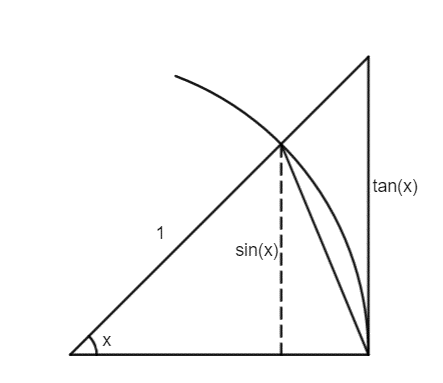
\includegraphics[scale =0.6]{DifferentialCalculusPictures/limitTriangle.png}
\begin{align*}
    &\text{Area of segment: }\frac{x}{2}\\
    &\text{Area of big triangle: }\frac{\tan x}{2}\\
    &\text{Area of small triangle: } \frac{\sin x}{2}\\
    &\frac{\sin x}{2}\leq\frac{x}{2}\leq\frac{\tan x}{2}\\
    &\frac{1}{\sin x}\leq\frac{1}{x}\leq\frac{1}{\tan x}\\
    &=\frac{\sin x}{\sin x}\leq\frac{\sin x}{x}\leq \frac{\sin x}{\tan x}\\
    &=1\leq\lim_{x\to 0}\frac{\sin x}{x}\leq\lim_{x\to 0}\cos x\\
    &\therefore\,\lim_{x\to 0}\frac{\sin x}{x}=1
\end{align*}
Ex2: $\lim\limits_{x\to 0}\frac{\cos x-1}{x}$
\begin{align*}
    \lim\limits_{x\to 0}\frac{\cos x-1}{x}&=\lim_{x\to 0}\frac{-2\sin^2\left(\frac{x}{2}\right)}{x}\\
    &=\lim_{\frac{x}{2}\to 0}\frac{-\sin^2\left(\frac{x}{2}\right)}{\frac{x}{2}}\\
    &=\lim_{\frac{x}{2}\to 0}-\sin\left(\frac{x}{2}\right)\frac{\sin\left(\frac{x}{2}\right)}{\frac{x}{2}}\\
    &=0
\end{align*}
Now, a more general case:
\begin{align*}
    \text{Ex3: }&\lim_{x\to 0}\frac{\sin(ax)}{x}\\
    &\text{We know }\lim_{x\to 0}\frac{\sin x}{x}=1\\
    &\text{and }ax\to 0\Longleftrightarrow x\to 0\\
    &\text{so }\lim_{x\to 0}\frac{\sin(ax)}{ax}=1\\
    &\Ra\lim_{x\to 0}\frac{\sin(ax)}{x}=a
\end{align*}

\subsubsection{Continuity}
A function is said to be continuous at a point $c$ if the following three conditions are satisfied:
\begin{enumerate}
    \item $f(c)$ exists
    \item $\lim\limits_{x\to c}f(x)$ exists
    \item $\lim\limits_{x\to c}f(x)=f(c)$
\end{enumerate}
If $f(x)$ and $g(x)$ are continuous then the composition of $f$ and $g$ is also continuous.\\
The conditions of the derivative state that the function must be continuous. So if the derivative of a function is continuous, the original function must also be continuous.\\
Note that a continuous function does not always give a continuous derivative.\\
Ex: Find a real number $a$ such that $f(x)$ is continuous 
\begin{align*}
    &f(x)=\left\{\begin{matrix}
    \frac{x^2-9}{x+a},\, x<-a\\
    x+3,\,x\geq-a
    \end{matrix}\right.\\
    &\text{We need }\lim_{x\to-a^-}\frac{x^2-9}{x+a}=\lim_{x\to-a^+}(x+3)=-a+3\\
    &\lim_{x\to -a^-}\frac{(x+3)(x-3)}{x+a}=-a+3\\
    &\frac{(-a+3)(-a-3)}{\lim\limits_{x\to-a^-}(x+a)}=a+3\\
    &\Ra-a-3=\lim_{x\to-a^-}(x+a)=0\\
    &\Ra a=-3
\end{align*}